\documentclass[11pt,a4paper]{article}

% ----------------------------------------------------------------------
%  Philips Document Flow (PDF) - Technical Manual
%  Compiles in Overleaf with pdfLaTeX (default engine).
% ----------------------------------------------------------------------

\usepackage[utf8]{inputenc}
\usepackage[T1]{fontenc}
\usepackage[english]{babel}
\usepackage{lmodern}
\usepackage[a4paper,margin=2.5cm]{geometry}
\usepackage{xcolor}
\usepackage{booktabs}
\usepackage{array}
\usepackage{ragged2e}
\usepackage{tabularx}
\usepackage{xltabular}
\usepackage{enumitem}
\usepackage{listings}
\usepackage{fancyhdr}
\usepackage{titlesec}
\usepackage{tikz}
\usetikzlibrary{arrows.meta,positioning}
\usepackage[hidelinks]{hyperref}

% ---- Sober palette (text always black) -------------------------------
\definecolor{codebg}{RGB}{246,247,248}
\definecolor{linegray}{RGB}{200,205,210}
\definecolor{headgray}{RGB}{238,240,242}
\color{black}

% ---- Code style (monochrome, black text) -----------------------------
\lstdefinestyle{code}{
  basicstyle=\ttfamily\small\color{black},
  backgroundcolor=\color{codebg},
  frame=single,
  rulecolor=\color{linegray},
  breaklines=true,
  showstringspaces=false,
  columns=fullflexible,
  keepspaces=true,
  captionpos=b,
  xleftmargin=6pt,
  xrightmargin=6pt,
  aboveskip=10pt,
  belowskip=6pt,
}
\lstset{style=code}

% ---- Table columns that wrap and do NOT overlap ----------------------
% L = flexible column, left-aligned text with line wrapping.
\newcolumntype{L}{>{\RaggedRight\arraybackslash}X}
\newcolumntype{C}{>{\Centering\arraybackslash}X}

% ---- Header and footer -----------------------------------------------
\pagestyle{fancy}
\fancyhf{}
\setlength{\headheight}{14pt}
\fancyhead[L]{\small\itshape Philips Document Flow (PDF) --- Technical Manual}
\fancyhead[R]{\small\thepage}
\renewcommand{\headrulewidth}{0.4pt}

% ---- Title formatting (black, with a thin rule) ----------------------
\titleformat{\section}
  {\Large\bfseries\color{black}}{\thesection}{0.6em}{}[\vspace{1pt}{\color{linegray}\titlerule}]
\titleformat{\subsection}{\large\bfseries\color{black}}{\thesubsection}{0.6em}{}
\titlespacing*{\section}{0pt}{16pt}{8pt}

% ---- Macros ----------------------------------------------------------
% Backslash with a line-break point, for long paths in tables.
\newcommand{\bs}{\textbackslash\allowbreak}
\newcommand{\ruta}[1]{\texttt{\small #1}}

\setlength{\parskip}{4pt}
\setlength{\parindent}{0pt}

\begin{document}

% ======================================================================
%  COVER
% ======================================================================
\begin{titlepage}
\centering
\vspace*{3cm}
{\color{black}\rule{\textwidth}{1.2pt}}\\[0.8cm]
{\Huge\bfseries Philips Document Flow (PDF)}\\[0.5cm]
{\LARGE Technical Manual}\\[0.4cm]
{\color{black}\rule{\textwidth}{1.2pt}}\\[2cm]

{\large Desktop application for the automatic opening of downloaded\\
PDF documents (work instructions WI / MPI)}\\[3cm]

\begin{tabular}{@{}r l@{}}
\textbf{Platform} & Microsoft Windows 10 / 11 (x64) \\[5pt]
\textbf{Technology} & .NET 8 --- Windows Forms (C\#) \\[5pt]
\textbf{Rendering engine} & Microsoft WebView2 (Chromium) \\[5pt]
\textbf{Application version} & 2.1.0 \\[5pt]
\textbf{Date} & June 2026 \\
\end{tabular}

\vfill
\end{titlepage}

% ======================================================================
\tableofcontents
\newpage

% ======================================================================
\section{Introduction}
% ======================================================================
Philips Document Flow (PDF) is a Windows desktop application that automates the
viewing of downloaded PDF documents. It runs silently in the system tray and
watches the user's Downloads folder; when a new document appears, it opens it in a
built-in viewer and, once the user is done reading it, deletes it automatically to
keep the folder clean.

The application targets environments where documents may be distributed in two
languages, identified by a suffix in the file name:

\begin{itemize}[leftmargin=1.4em,itemsep=2pt]
  \item \texttt{\_SPA} --- document in Spanish.
  \item \texttt{\_ENG} --- document in English.
\end{itemize}

The design is deliberately narrow: the system only \textbf{watches},
\textbf{opens}, \textbf{closes after use} and \textbf{deletes} the documents. It
performs no other action on the machine or on the user's data.

% ======================================================================
\section{Key features}
% ======================================================================
\begin{itemize}[leftmargin=1.4em,itemsep=3pt]
  \item Automatic opening of downloaded PDFs, with no user intervention.
  \item A dedicated built-in viewer based on the WebView2 (Chromium) engine.
  \item Automatic deletion of the document when it is closed.
  \item A 20-minute viewing limit, with a prior warning at 15 minutes.
  \item Automatic replacement of a document by its most recent copy.
  \item A configurable language filter when both versions are downloaded.
  \item Robust download detection via file-system events and a periodic
        backup rescan.
  \item Its own visual identity: a blue icon with the text ``PDF'' applied to the
        executable, the window, the taskbar and the system tray.
  \item English user interface, as the standard for use across different plants.
\end{itemize}

% ======================================================================
\section{System architecture}
% ======================================================================
The application is organized in two layers: a logic layer (\texttt{Core}) and a
user-interface layer (\texttt{UI}). There is no permanent main window; the
application's point of persistence is the system-tray icon.

\vspace{0.4cm}
\begin{center}
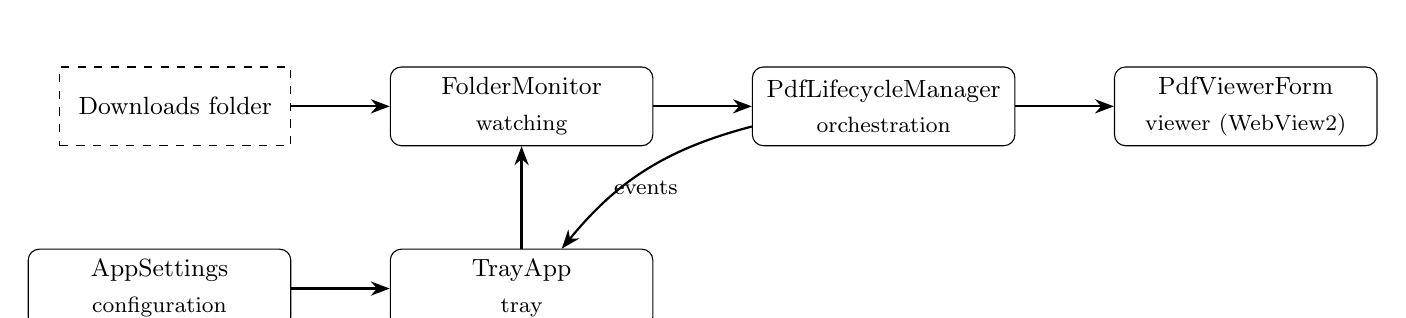
\begin{tikzpicture}[
  node distance=0.85cm and 1.25cm,
  every node/.style={font=\small},
  comp/.style={rectangle, rounded corners, draw=black, fill=white,
               text width=3.1cm, align=center, minimum height=1.0cm},
  ext/.style={rectangle, draw=black, dashed, fill=white, text width=2.7cm,
              align=center, minimum height=1.0cm},
  arr/.style={-{Stealth[length=2.4mm]}, thick}
]
\node[ext]  (fs)   {Downloads folder};
\node[comp] (mon)  [right=of fs]  {FolderMonitor\\[2pt]\footnotesize watching};
\node[comp] (life) [right=of mon] {PdfLifecycleManager\\[2pt]\footnotesize orchestration};
\node[comp] (view) [right=of life]{PdfViewerForm\\[2pt]\footnotesize viewer (WebView2)};
\node[comp] (tray) [below=1.3cm of mon] {TrayApp\\[2pt]\footnotesize tray};
\node[comp] (set)  [left=of tray] {AppSettings\\[2pt]\footnotesize configuration};

\draw[arr] (fs)   -- (mon);
\draw[arr] (mon)  -- (life);
\draw[arr] (life) -- (view);
\draw[arr] (set)  -- (tray);
\draw[arr] (tray) -- (mon);
\draw[arr] (life) to[bend right=18] node[midway,below,font=\footnotesize]{events} (tray);
\end{tikzpicture}
\end{center}
\vspace{0.3cm}

\begin{xltabular}{\textwidth}{@{} >{\bfseries}p{5.1cm} L @{}}
\toprule
\normalfont\textbf{Component} & \textbf{Responsibility} \\
\midrule
\endfirsthead
\toprule
\normalfont\textbf{Component} & \textbf{Responsibility} \\
\midrule
\endhead
\bottomrule
\endfoot
Program & Entry point. Initializes the application context. \\
TrayApp & Keeps the application alive through the tray icon and wires the components together. \\
AppSettings & Loads and saves the user configuration in JSON format. \\
FolderMonitor & Detects the appearance of new PDF files in the watched folder. \\
PdfLifecycleManager & Orchestrates the full lifecycle of each detected document. \\
PdfViewerForm & Built-in viewer based on WebView2; displays the PDF and controls its closing. \\
StatusForm & Main window: monitor status and language selection. \\
\bottomrule
\end{xltabular}

% ======================================================================
\section{Processing flow}
% ======================================================================
Each detected document is processed in an independent background task, so that
multiple simultaneous downloads do not block one another. The cycle consists of
the following stages:

\begin{enumerate}[leftmargin=1.6em,itemsep=3pt]
  \item \textbf{Detection.} The watched folder reports the appearance of a file
        with a \texttt{.pdf} extension.
  \item \textbf{Stabilization.} The application waits for the browser to finish
        writing the file, checking that the size stays stable and that no process
        holds a write lock.
  \item \textbf{Opening.} The document is opened in the built-in viewer.
  \item \textbf{Wait.} The cycle blocks until the window closes, whether by the
        user, by the replacement with a more recent copy, by the language filter,
        or by the 20-minute limit.
  \item \textbf{Deletion.} The file is deleted safely.
\end{enumerate}

\subsection{Duplicate control and reprocessing}
The application keeps several in-memory structures to ensure that each document is
processed only once and that no download is lost:

\begin{itemize}[leftmargin=1.4em,itemsep=2pt]
  \item \textbf{In progress:} paths currently being processed.
  \item \textbf{Cooldown:} recently finished paths, to ignore late file-system
        events.
  \item \textbf{Handled:} paths already attended to, together with their
        modification date, so as not to reopen a document that has not changed.
\end{itemize}

% ======================================================================
\section{Download detection}
% ======================================================================
The detection of new files combines two complementary mechanisms that, together,
guarantee that no document is left unopened.

\subsection{File-system events}
The \texttt{FolderMonitor} component uses the standard .NET
\texttt{FileSystemWatcher} class, which immediately reports file creation and
renaming. Browsers download to a temporary file (for example \texttt{.crdownload})
and rename it to \texttt{.pdf} once the download completes; both cases are
detected.

\subsection{Periodic backup rescan}
As a safety net against lost events (system buffer overflow or browser race
conditions), a timer rescans the folder every three seconds and reconsiders any
PDF modified within the last three minutes. The memory of already-processed
documents prevents an open file from being reopened.

% ======================================================================
\section{Built-in viewer}
% ======================================================================
Documents are always opened in a dedicated viewer based on \textbf{Microsoft
WebView2}, the Chromium PDF rendering engine shipped with Windows. The viewer has
the following characteristics:

\begin{itemize}[leftmargin=1.4em,itemsep=2pt]
  \item It loads local paths exclusively, via the \texttt{file://} scheme; it does
        not navigate to Internet addresses.
  \item Exact close detection through the window's own close event.
  \item Fast opening: a WebView2 process is kept warm in the background so that
        each document opens without the delay of a cold start.
  \item Each window runs on its own thread, which allows several documents to be
        displayed independently.
\end{itemize}

% ======================================================================
\section{Language filtering}
% ======================================================================
The file name determines its language through the \texttt{\_SPA} and \texttt{\_ENG}
suffixes. The behavior depends on how many documents are downloaded and on the
configured preference.

\begin{xltabular}{\textwidth}{@{} L L @{}}
\toprule
\textbf{Situation} & \textbf{Behavior} \\
\midrule
\endfirsthead
\toprule
\textbf{Situation} & \textbf{Behavior} \\
\midrule
\endhead
\bottomrule
\endfoot
A single document (with or without a language suffix) & Always opens. \\
Two documents, no preferred language & Both open. \\
Two documents, with a preferred language & Both open and, once visible, the
non-matching one closes automatically; the preferred language remains. \\
\bottomrule
\end{xltabular}

\subsection{Document pairing}
Two files are considered the same document in different languages when, after
removing the language suffix and normalizing the separators, they share the same
base name. For example, \texttt{D000\_H\_SPA\_Report} and
\texttt{D000\_H\_ENG Report} are paired correctly.

% ======================================================================
\section{Replacement by a more recent copy}
% ======================================================================
If a document is already open and the user downloads a more recent copy of the
same document in the same language (for example \texttt{report (1).pdf} while
\texttt{report.pdf} is on screen), the application closes the previous copy's
window and shows the new one. This way the operator always sees the most recent
version.

Because the new copy opens in a new window, the 20-minute viewing limit restarts
automatically. The previous copy is deleted when it closes, while the copy in use
is protected against that deletion.

% ======================================================================
\section{Viewing time limit}
% ======================================================================
Each document may stay open for a maximum of \textbf{20 minutes}. The control is
as follows:

\begin{itemize}[leftmargin=1.4em,itemsep=2pt]
  \item At \textbf{15 minutes} a notification warns that the document will close in
        5 minutes.
  \item At \textbf{20 minutes} the window closes automatically and the document is
        deleted as on any close.
\end{itemize}

This time notification is the only routine notification the application raises.

% ======================================================================
\section{File deletion}
% ======================================================================
Deletion is restricted exclusively to the watched folder and runs after each
document is closed. The process accounts for the usual temporary locks (antivirus
scanning, folder synchronization, the viewer itself):

\begin{itemize}[leftmargin=1.4em,itemsep=2pt]
  \item \textbf{Immediate retries:} each deletion is retried at growing intervals
        for about nine seconds.
  \item \textbf{Background cleanup:} if the file is still locked, it is recorded in
        a pending list that is retried periodically until it completes; no file is
        silently left undeleted.
  \item \textbf{Re-download protection:} if a pending file changes (because it was
        downloaded again), it is removed from the list and processed as a new
        document, avoiding the deletion of current content.
\end{itemize}

In addition, the application recognizes the duplicate copies that browsers
generate (for example, \texttt{document (2).pdf}) and includes them in the cleanup
of the corresponding document.

% ======================================================================
\section{Configuration}
% ======================================================================
The only user-configurable option is the \textbf{preferred language}, selected
from the application's main window. The rest of the behavior is fixed by design:
the watched folder, the use of the built-in viewer, the automatic deletion and the
20-minute limit.

The configuration is saved in JSON format, in readable text:

\begin{lstlisting}[caption={Example settings.json.}]
{
  "PreferredLanguage": "SPA"
}
\end{lstlisting}

If the file does not exist or is corrupt, the application falls back to safe
defaults.

\begin{xltabular}{\textwidth}{@{} >{\bfseries}p{3.4cm} p{2.2cm} L @{}}
\toprule
\normalfont\textbf{Parameter} & \textbf{Values} & \textbf{Description} \\
\midrule
\endfirsthead
\toprule
\normalfont\textbf{Parameter} & \textbf{Values} & \textbf{Description} \\
\midrule
\endhead
\bottomrule
\endfoot
PreferredLanguage & Any, SPA, ENG & Language opened when both versions are
downloaded at once. \texttt{Any} opens both. \\
\bottomrule
\end{xltabular}

% ======================================================================
\section{Data storage}
% ======================================================================
The application stores its data in the user's local folder, without affecting
other users of the machine.

\begin{xltabular}{\textwidth}{@{} L p{4.2cm} @{}}
\toprule
\textbf{Path} & \textbf{Content} \\
\midrule
\endfirsthead
\toprule
\textbf{Path} & \textbf{Content} \\
\midrule
\endhead
\bottomrule
\endfoot
\ruta{\%LOCALAPPDATA\%\bs PdfAutoViewer\bs settings.json} & User configuration. \\
\ruta{\%LOCALAPPDATA\%\bs PdfAutoViewer\bs WebView2\bs} & Working data of the built-in viewer. \\
\ruta{\%LOCALAPPDATA\%\bs PdfAutoViewer\bs viewer-error.log} & Viewer diagnostic log, if applicable. \\
\ruta{\%LOCALAPPDATA\%\bs PdfAutoViewer\bs app-error.log} & Log of unhandled exceptions, if applicable. \\
\bottomrule
\end{xltabular}

% ======================================================================
\section{System requirements}
% ======================================================================
\begin{itemize}[leftmargin=1.4em,itemsep=2pt]
  \item Microsoft Windows 10 or 11 (64-bit).
  \item .NET 8 Desktop Runtime.
  \item WebView2 Runtime (included by default on Windows 11).
\end{itemize}

% ======================================================================
\section{Build and run}
% ======================================================================
The project is built with the .NET 8 SDK.

\begin{lstlisting}[caption={Build and run.}]
# Run in development mode
dotnet run --project PdfAutoViewer/PdfAutoViewer.csproj

# Build in Release mode
dotnet build -c Release

# Publish a single-file executable
dotnet publish PdfAutoViewer/PdfAutoViewer.csproj -c Release ^
       -r win-x64 --self-contained false -o publish
\end{lstlisting}

The \texttt{PdfAutoViewer.sln} solution can also be opened in Visual Studio 2022 or
JetBrains Rider.

\subsection{Installing the SDK without administrator privileges}
On corporate machines without administrator rights, the .NET 8 SDK can be
installed per-user, under \ruta{\%USERPROFILE\%\bs.dotnet}, and used by its full
path. From the Visual Studio Code integrated terminal (PowerShell), at the project
root:

\begin{lstlisting}[caption={Running with a local SDK (no administrator).}]
& "$env:USERPROFILE\.dotnet\dotnet.exe" run --project PdfAutoViewer
& "$env:USERPROFILE\.dotnet\dotnet.exe" test PdfAutoViewer.Tests
\end{lstlisting}

\subsection{Versioning}
The application version is defined once in the project file
(\texttt{PdfAutoViewer.csproj}, the \texttt{<Version>} tag) and the status window
reads it at runtime from the assembly. To release a new version it is enough to
update that value; no code changes are required.

The application allows a single instance per Windows session: if a copy is already
running in the same session, a new launch closes immediately. In multi-session
environments (VDI or multi-session hosts), each session runs its own independent
instance.

% ======================================================================
\section{Dependencies}
% ======================================================================
\begin{xltabular}{\textwidth}{@{} >{\bfseries}p{5.2cm} p{2.4cm} L @{}}
\toprule
\normalfont\textbf{Dependency} & \textbf{Version} & \textbf{Role} \\
\midrule
\endfirsthead
\toprule
\normalfont\textbf{Dependency} & \textbf{Version} & \textbf{Role} \\
\midrule
\endhead
\bottomrule
\endfoot
.NET (Windows Desktop) & 8.0 & Execution platform. \\
Windows Forms & 8.0 & User interface. \\
Microsoft.Web.WebView2 & 1.0.x & Built-in viewer engine. \\
WebView2 Runtime & System & Operating-system component. \\
\bottomrule
\end{xltabular}

The only external package dependency is \texttt{Microsoft.Web.WebView2}; all
dependencies are official Microsoft components.

% ======================================================================
\section{Security and privacy}
% ======================================================================
The application \textbf{does not establish network connections}. It includes no
HTTP client libraries or telemetry mechanisms, and the built-in viewer loads only
local files via the \texttt{file://} scheme. It does not collect, store or
transmit user information or document content; from each file, only its name and
size are read.

The following table lists the operating-system resources the application uses,
with its access level.

\begin{xltabular}{\textwidth}{@{} >{\bfseries}p{4.3cm} p{2.8cm} L @{}}
\toprule
\normalfont\textbf{Resource} & \textbf{Access} & \textbf{Use} \\
\midrule
\endfirsthead
\toprule
\normalfont\textbf{Resource} & \textbf{Access} & \textbf{Use} \\
\midrule
\endhead
\bottomrule
\endfoot
Windows Registry & Read & Resolving the path of the user's Downloads folder. \\
Watched folder & Read / Delete & PDF detection, size reading and deletion after use. \\
App data folder & Read / Write & Configuration and WebView2 working data. \\
Processes & Indirect & The WebView2 engine runs PDF rendering in its own processes managed by its runtime. \\
Network & None & The application makes no network connections. \\
\bottomrule
\end{xltabular}

It runs with the privileges of the user who starts it; it requires no
administrator elevation, installs no services or drivers and changes no system
settings. Its file operations are limited to the watched folder and its own data
folder.

% ======================================================================
\section{Error handling and logging}
% ======================================================================
The application is designed to degrade gracefully:

\begin{itemize}[leftmargin=1.4em,itemsep=2pt]
  \item If a deletion fails due to a temporary lock, it is retried in the
        background without interrupting operation.
  \item Relevant errors are reported through a system-tray notification, so a
        failure does not go unnoticed.
  \item The viewer logs initialization failures to a local diagnostic file to ease
        support.
  \item Unhandled exceptions are logged to a local diagnostic file; those on the
        UI thread are caught so that a one-off error does not stop the
        application.
\end{itemize}

% ======================================================================
\section{Known limitations}
% ======================================================================
\begin{itemize}[leftmargin=1.4em,itemsep=3pt]
  \item Language filtering is only activated when both versions are downloaded
        almost simultaneously; downloads separated in time are treated as
        independent documents.
  \item Replacement by a more recent copy applies to documents of the same
        language; a version in another language is handled through the language
        filter.
\end{itemize}

% ======================================================================
\section{Version history}
% ======================================================================
\begin{xltabular}{\textwidth}{@{} p{1.8cm} p{2.6cm} L @{}}
\toprule
\textbf{Version} & \textbf{Date} & \textbf{Changes} \\
\midrule
\endfirsthead
\toprule
\textbf{Version} & \textbf{Date} & \textbf{Changes} \\
\midrule
\endhead
\bottomrule
\endfoot
2.1.0 & June 2026 & ``Philips Document Flow (PDF)'' branding; blue ``PDF'' icon on the executable, the window and the tray; fully English UI; version read from the assembly; technical manual in Spanish and English. \\
2.0 & --- & Single built-in viewer (WebView2); minimal configuration; 20-minute viewing limit; robustness for continuous operation. \\
\bottomrule
\end{xltabular}

\end{document}
